%%%%%%%%%%%%%%%%%%%%%%%%%%%%%%%%%%%%%%%%%%%%%%%%%%%
%%% ESTADO DEL ARTE
%%%%%%%%%%%%%%%%%%%%%%%%%%%%%%%%%%%%%%%%%%%%%%%%%%%

\chapter{State of the Art}
\fancyhead[RE]{\textsc{Chapter} \thechapter. State of the art}
\label{ch:StateOfTheArt}
\noindent Although both language models and explainability are young techniques, both of them have awaken the interest of the researchers and, therefore, there are a lot of works regarding to these areas of research.
\paragraph{}
In this section, the state of the art of the language models, the question answering task and the explainability is being reviewed, from the history to the most novel methods, seeing the evaluation methods and \emph{datasets} available and the most interesting papers.
\section{Language models}
\label{sec:LanguageModels}
\noindent In 2001, Joshua Bengio et al. proposed the first neural language model, based on a feed-forward neural network.\cite{Bengio2001} However, it wasn't until 2013 that neural networks begin to gain relevance in the world of \emph{NLP}, and it was due to the \emph{word embeddings} and the new neural architectures, like \emph{Recurrent Neural Networks} (\emph{RNN}).
\paragraph{}
The \emph{word embeddings} are vectorized representantions of the words contained in a document, and since its begining have gained a lot of importance in the world of the \emph{NLP}, because they are able to capture the context of the word within the text, improving the way the model understands the text. This way, a polysemic word has not the same representation in different contexts. One example of this techinque is \emph{Word2Vec}, probably the most used technique by the researchers to learn the \emph{word embeddings} of the text, and was developed by Tomas Mikolov in 2013.\cite{Mikolov2013}.
\begin{figure}[h!]
	\centering
	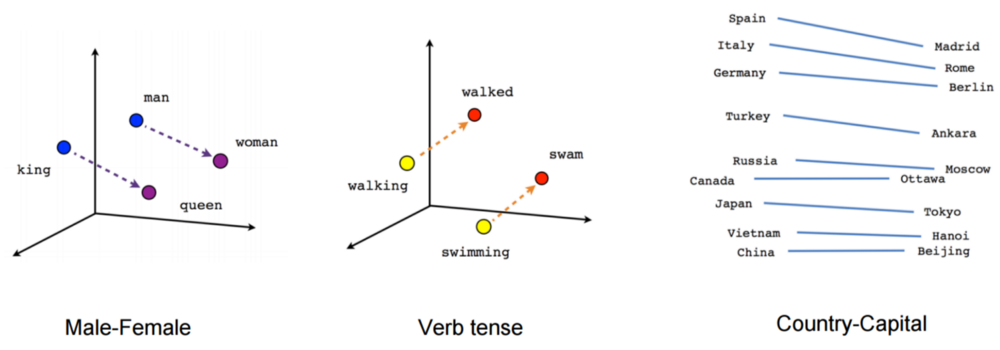
\includegraphics[scale=0.35]{images/wordembeddings}
	\caption{Word Embeddings}
	\label{fig:wordembdedding}
\end{figure}
\paragraph{}
When dealing with temporal series or data sequences, neural networks are not able to model the temporal dependency, as they don't have knowledge about the previous sequences. To solve this, a new variety of neural networks was developed, the \emph{RNN}, that have the ability to process data sequences by saving memory of the already processed ones. In \emph{NLP} this is really important, because in natural language texts a single word is not enough to capture its meaning, also the previous words (or sentences) are needed, so the ability to save ``memory'' about the previous words improved the performance of neural networks in almost every \emph{NLP} task. Thus, a lot of versions of neural networks have been developed, like the \emph{Long Short-Term Memories} (\emph{LSTM}), that are very used in \emph{NLP} because they save the memory during more time than other versions, increasing the window size of the sequences being seen.
\begin{figure}[!h]
	\centering
	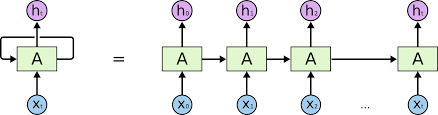
\includegraphics[scale=0.55]{images/lstm}
	\caption{\emph{LSTM} Recurrent Neural Networks.}
	\label{fig:lstm}
\end{figure}
\paragraph{}
Other architecture that has revolutionized the research world in \emph{NLP}, contributing to the appearance of new language models is the \emph{encoder-decoder} architecture, based on two different parts, the \emph{encoder} that codifies the input, getting a vectorized representation that is transmitted to the second part, the \emph{decoder}, that from this codified sate generates the output. Usually, a sentence is given as input and the output is a new sentence, so that this architecture is also known as \emph{sequence to sequence}. In its beginning it was used to \emph{machine translation} task, having as input a text in some language and the translation as output.
\begin{figure}[h!]
	\centering
	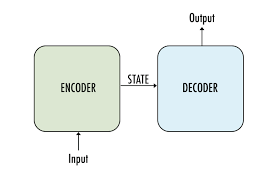
\includegraphics[scale=0.75]{images/encoderdecoder}
	\caption{\emph{Encoder-Decoder} architecture.}
	\label{fig:encoderdecoder}
\end{figure}
\paragraph{}
One of the main problems of this architecture is the need of codify the whole input before the output generation, that is done by looking at the whole input. The \emph{attention} mechanism was developed to solve this, giving as input for the \emph{decoder} not only the codified state of the input (as in the classic \emph{encoder-decoder} architecture) but also the hidden states of the \emph{encoder}, that now process the input splitted, making possible to look only at one part of the input and not the whole input as before.\cite{Bahdanau2014} 
\begin{figure}[h!]
	\centering
	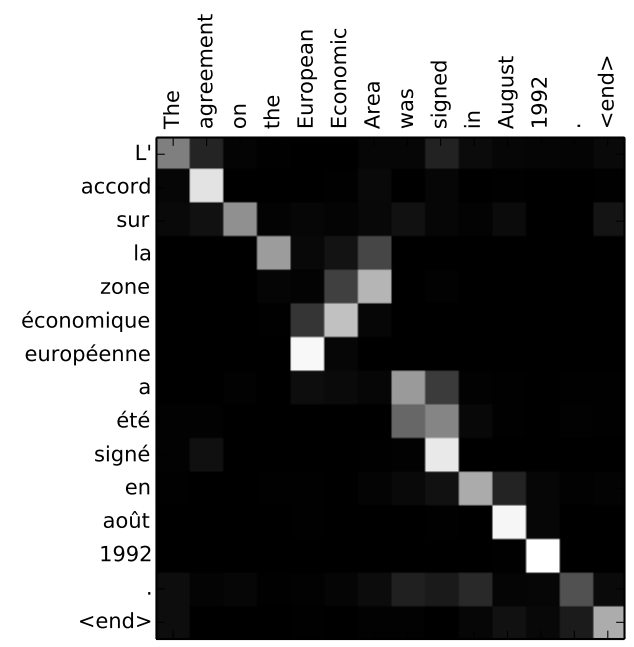
\includegraphics[scale=0.35]{images/attention}
	\caption{Example of the \emph{Attention} mechanism in machine translation. It can be seen as the \emph{Attention} mechanism focus only on the words being translated and the relevant ones instead in the whole sentence.}
	\label{fig:attention}
\end{figure}
\paragraph{}
Three years later, in 2017, probably the most important article in the history of \emph{NLP} was released: ``Attention is all you need''.\cite{Vaswani2017} In the article, Vaswani et al. propose a novel neural architecture based only on layers using the \emph{Attention} mechanism, the \emph{Transformer}. Besides, the \emph{Transformers} use a variation of the \emph{Attention} mechanism called \emph{Self-Attention}, that allows to take as input other positions of the self input, which makes possible to use other words of the same input to codify each word, as can be seen in Figure \ref{fig:selfattention}.
\begin{figure}[h!]
	\centering
	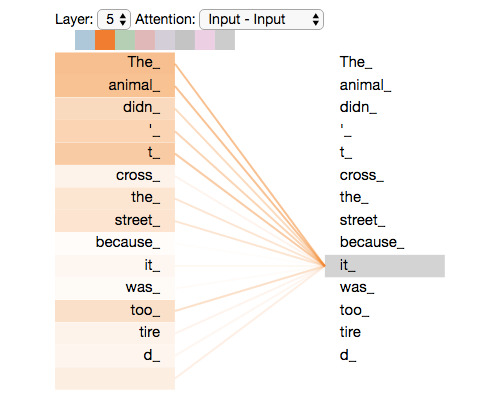
\includegraphics[scale=0.45]{images/selfattention}
	\caption{\emph{Self-Attention} mechanism.}
	\label{fig:selfattention}
\end{figure}
\paragraph{}
In the \emph{Transformer}, the output of different \emph{Self-Attention} layers are concatenated, creating a multi-dimensional \emph{Attention} representation, what is the \emph{Multi-Head Attention}. This way, each head can learn to codify the same word in different ways, what allows the model to capture more information of the word. Although it can be considered as \emph{Transformer} every architecture designed to process a set of words with the \emph{Attention} mechanism as the unique way of interaction between them, the basic structure of the \emph{Transformer} is based on:
\begin{itemize}
\item \emph{Self-Attention} or \emph{Multi-head Attention} layer.
\item Normalization layer.
\item \emph{Feed-forward} layer.
\item Normalization layer.
\item Residual connections.
\end{itemize}
With this, an \emph{encoder-decoder} architecture is developed, as shown in Figure \ref{fig:transformer}.
\begin{figure}[h!]
	\centering
	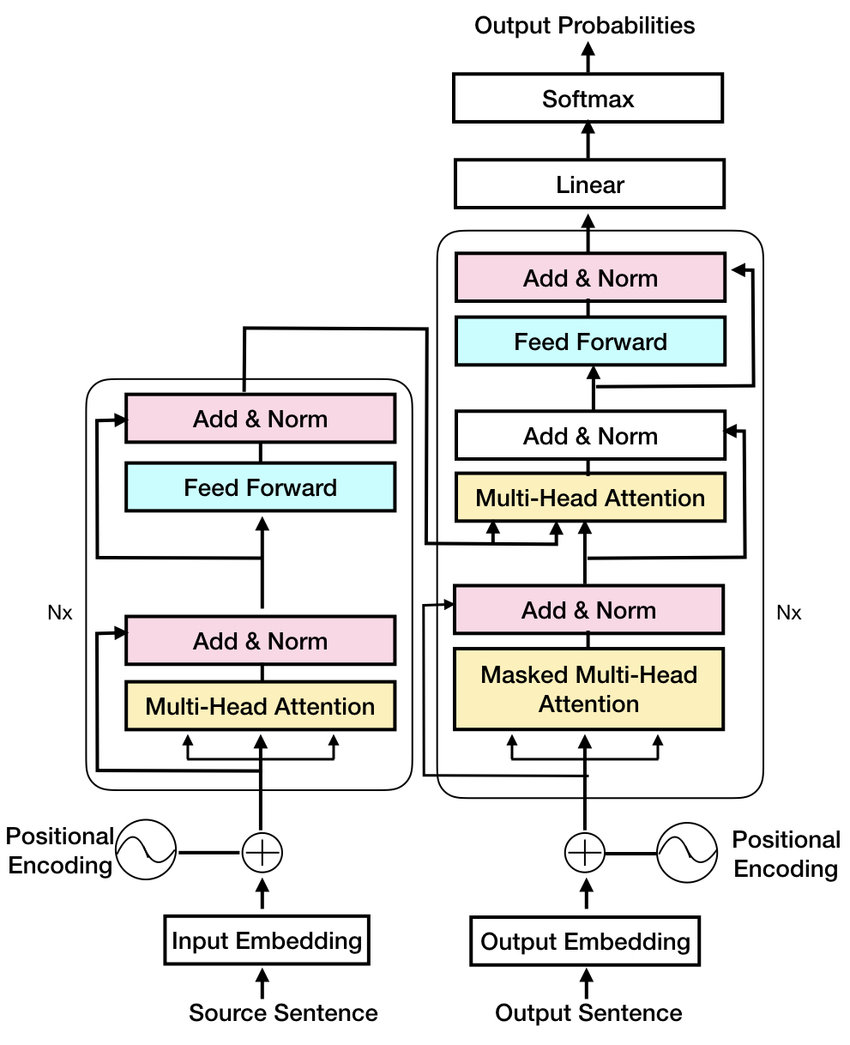
\includegraphics[scale=0.25]{images/transformer}
	\caption{\emph{Transformer} architecture.}
	\label{fig:transformer}
\end{figure}
\paragraph{}
Another one of the key points to the massive expansion of the language models has been the training techniques used. Along the history of the language models, they used to be unidirectionals, this is, to predict the next word they used only the words before. But this changed with the arrival of \emph{BERT}, \emph{Pre\-training of Deep Bidirectional Transformers for Language Understanding}. \cite{Devlin2018} Instead of predict the next word, \emph{BERT} masks randomly some tokens in the input, and trains by trying to predict the original words that have been masked, using both left and right sides of the sentences (bidirectional), which allows the model to capture more information while codifying the tokens. This is known as \emph{Masked Language Models}, \emph{MLM}.
\paragraph{}
Although the most common way to work is dealing with words, the language models can work in different ways, like for example using \emph{n-grams} and using smooth techniques to deal with \emph{n-grams} neer seen before\cite{Knesser1995}. Another ones, like \emph{ProphetNet} \cite{Yan2020}, try to predict not only the next token, but the $n$ following tokens.
\paragraph{}
So, the basic idea behind the language models is to predict the next token, but they can be used also for other \emph{NLP} tasks such as \emph{Question Answering}. To achieve this, different additional layers are set on top of the language model, trained to solve the specific task, taking as input the output of the language model, this is, the original input tokenized. 
\paragraph{}
Therefore, there are two different parts, the language model and the specific layers, and there are also two different types of training, the one used to train the language model (without the specific layers), that can be trained using massive amounts of texts, like the \emph{Wikipedia}, and the one used to train the model to the specific task, which requires a specific \emph{dataset}, which is known as \emph{fine-tuning}.
\subsection{Main Language Models for Question Answering}
\noindent Since the release of \emph{BERT} the number of papers and models published has suffered an exponential grown, Figure \ref{fig:cronology}, most of them using the same architecture than \emph{BERT}, or with little variations.
\begin{figure}[h!]
	\centering
	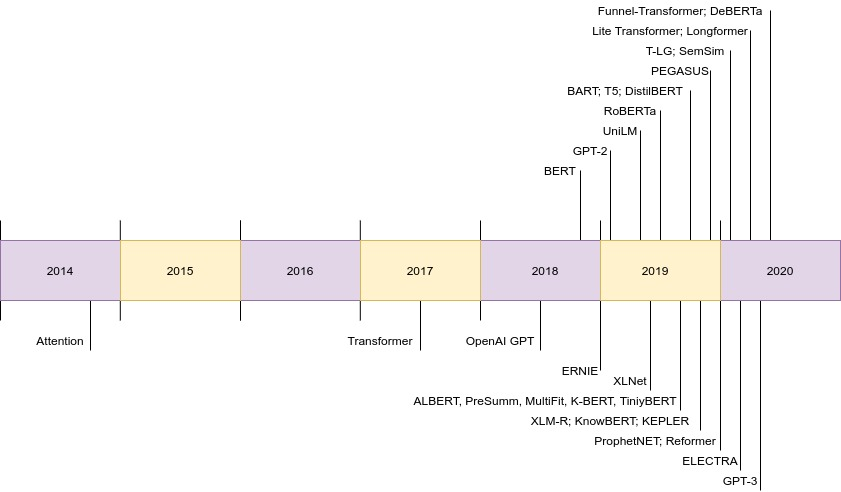
\includegraphics[scale=0.35]{images/cronology}
	\caption{Chronological view of a sample of language models. It can be seen that since \emph{BERT} the number of language models released has grown exponentially.}
	\label{fig:cronology}
\end{figure}
So, after a research of the state of the art of language models, it has been developed a brief review of some of the most interesting models.
\subsubsection{BERT}
\noindent As said before, the ``boom'' of the \emph{LM} started with \emph{BERT}, \emph{Pre\-training of Deep Bidirectional Transformers for Language Understanding}\cite{Devlin2018}. In this article, Devlin et al. propose a novel architecture based on the classic \emph{encoder-decoder} but, in this case, made only with \emph{Transformers}. There were released two different versions of \emph{BERT} depending on its size: one with 12 layers and 110 million parameters (the same as the \emph{OpenAI GPT} for comparison purposes); and one with 24 layers and a total number of 340 million parameters.
\paragraph{}
The \emph{WordPiece} embeddings (\cite{Wu2016}) are used, with a total umber of 30.000 \emph{tokens} in the vocabulary. The first \emph{token} of each sequence (understanding as sequence not a sentence of the text, but the input given to \emph{BERT} than can be up to two sentences) is a \emph{{CLS} token}, sentences in the input sequence are separated by a \emph{[SEP] token}.
\paragraph{}
In addition to this, a (not) new training is used, in which some random \emph{tokens} are masked (replaced by a \emph{[MASK] token}), and the model has to predict which one was the original \emph{token}. Altough this method started to be famous thanks to \emph{BERT} it wasn't invented by Devlin et al., but it was known as \emph{Cloze} task in the literature \cite{Taylor1953}. In the article, the authors explain that while training \emph{BERT} a 15\% of the \emph{tokens} is `masked''. When masking a \emph{token}, there are 3 possibilities:
\begin{enumerate}
\item The \emph{token} is replaced by a \emph{[MASK] token} 80\% of the time.
\item The \emph{token} is replaced by a random \emph{token} 10\% of the time.
\item The \emph{token} is not changed 10\% of the time.
\end{enumerate}
But this is not the only way \emph{BERT} is trained. It is also trained for another task, the prediction of the next sentence, \emph{NSP} (Next Sentence Prediction). In this task, two sentences are selected from the text ($A$ and $B$). 50\% of the time $B$ is the sentence that really follows $A$, meanwhile a 50\% of the time is not. In this task $BERT$ has to classify if $B$ is the next sentence following $A$ or not. 
\subsubsection{T5}
\noindent \emph{T5}, created by Raffel et al. in Google, in 2019.\cite{Raffel2019} is a model proposed in an extense research article with multiple tests of different architectures based on \emph{Transformers} and with a mask training, the same used by \emph{BERT}.
\paragraph{}
Besides the high-quality research presented, \emph{T5} does not propose any novel architecture, but due to its high size and its training over a really big \emph{corpus} obtained from the \emph{World Wide Web} (known as \emph{C4}, \emph{Colossal Clean Crawled Corpus}), \emph{T5} obtains state-of-the-art performance in multiple \emph{NLP} tasks, such as \emph{Question Answering}.
\subsubsection{GPT-2/GPT-3}
\emph{GPT} architectures, \cite{Openai}\cite{Radford2019}\cite{Brown2020}, are a group of language models based on an architecture based only on \emph{decoders}, without the encoder that is habitual in language models. These decoders layers are trained predicting next words, without a masked training, as it used to be in the past, which is known as ``from left to right''. This way, the model can only see the words at the left of the token being processed, loosing some of the context, but the quality of the generated text in \emph{Natural Language Generation} (\emph{NLG}) tasks is usually of a higher quality, because in runtime while generating new text, the model can only see the text at the left of the word.
\begin{figure}[h!]
	\centering
	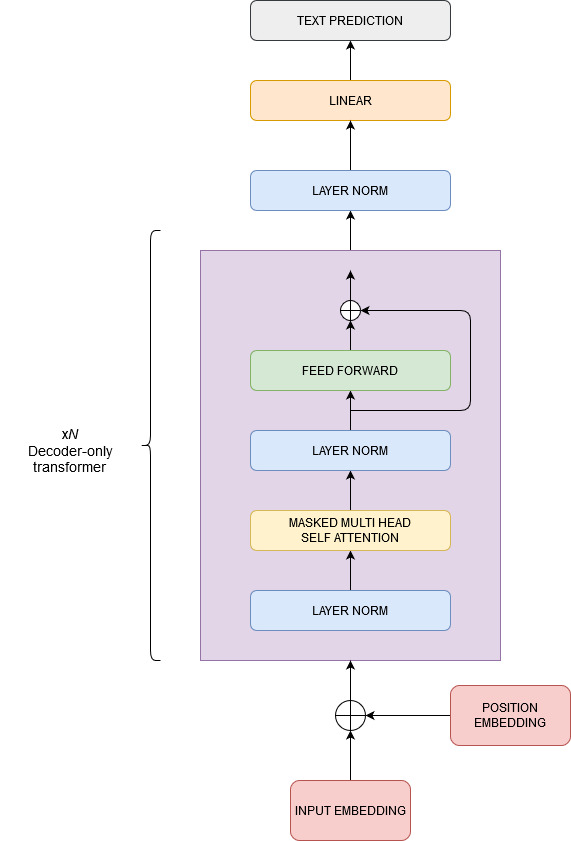
\includegraphics[scale=0.45]{images/gpt2}
	\caption{\emph{GPT-2} architecture.}
	\label{fig:gpt2}
\end{figure}
\paragraph{}
\emph{GPT-2} architecture caused quite a stir among all the researchers in \emph{NLP} (and also in the news), due to the quality of its generated text. But it also demonstrated that \emph{LM} are able to generalize and solve tasks without a specific \emph{fine-tuning} for the task. This way, \emph{GPT-2} was trained on a huge \emph{corpus}, but it was not trained for a specific training such as \emph{QA}. Even when the results are not as good in the benchmarks as the ones obtained from other models trained specifically for the task, results are really good, especially in \emph{NLG} tasks, which is surprisingly due to the fact that the model has not been trained for that.
\paragraph{}
The \emph{dataset} used to train \emph{GPT-2} is known as \emph{WebText}, and was generated from posts of the social network \emph{Redit}. To assure a good quality of these posts, only those who had a high punctuation were used, obtaining this way a set of texts well-written and covering different topics.
\paragraph{}
But, again, it wasn't trained for a specific tasks. Nevertheless, posts in \emph{Redit} are written by real people interacting with each other, so the model has been able to learn how to solve different tasks of \emph{NLP}. For example, in these posts some users made a question that other users answered, and this way the model learned to answer questions. 
\paragraph{}
Other interesting example is for the \emph{Text Summarization} (\emph{TS}) task, which consists on generate an abstract from a text. In these posts, users used to add a brief summary at the end of the post, tagged with the acronym \emph{TL;DR:} (Too Large; Didn't Read:). Researchers found that if this token is added to the model at the end of the input, the text generated by \emph{GPT-2} is the summary of the input, solving the \emph{TS} task.
\paragraph{}
When \emph{GPT-2} was released its large size was surprised (1.542 millions - 48 \emph{decoder} layers), which makes possible to understand the text and to generate a high quality output. But now the size of \emph{GPT-2} is not even close to the largest models used in \emph{NLP}.
\paragraph{}
Its ``big brother'', \emph{GPT-3}, its the largest model by the date of this article, with 175.000 millions of parameters, what allows it to understand the language in a way never seen before. Its able to solve any task in any domain without needing to adapt it with a specific \emph{fine-tunnning}, which is known as \emph{zero-shot}.
\paragraph{}
Its also able to solve, not only \emph{NLP} tasks, but also even arithmetic operations up to 3 digits, something really impressive that demonstrates its knowledge beyond the languages.
\subsubsection{Turing NLG}
\noindent \emph{Turing NLG} or \emph{T-NLG}\cite{Rosset2020} its a model developed by \emph{Microsoft} and, till the release of \emph{GPT-3} was the largest model published, with 17.000 millions of parameters (10 times less than \emph{GPT-3}). Nevertheless, its still a really massive amount of parameters, which allows \emph{T-NLG} to reach state-of-the-art performance in almost any \emph{NLP} task, such \emph{QA} or \emph{TS}.
\paragraph{}
Due to it large size, the \emph{Microsoft} team developed a \emph{Deep Learning} library (\emph{DeepSpeed}) and a new optimizer (\emph{ZeRo}) that allow the parallelization in the optimization and reduce the resources needed by the model to make possible the training of large models in a more efficient way, with less resources.
\begin{figure}[h!]
	\centering
	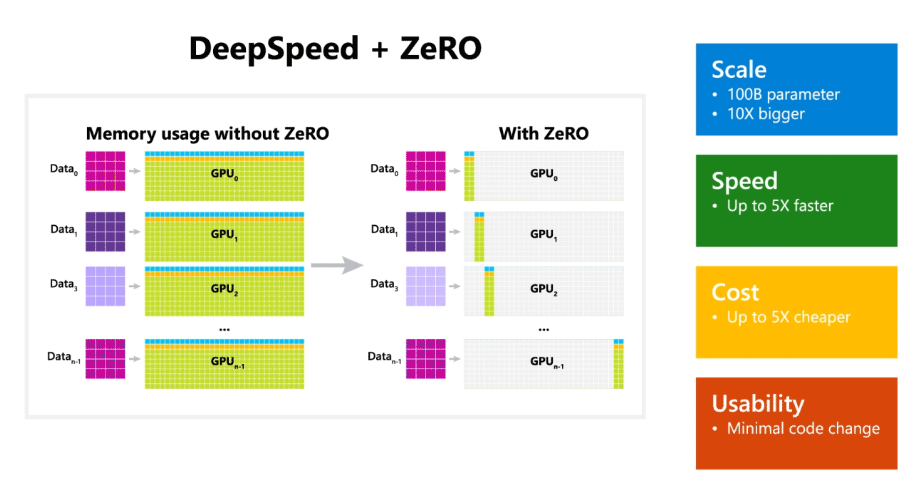
\includegraphics[scale=0.35]{images/tnlg}
	\caption{\emph{T-NLG}, \emph{DeepSpeed} and \emph{ZeRo}.}
	\label{fig:tnlg}
\end{figure}
\paragraph{}
In addition, \emph{T-NLG} has demonstrated that, as large is the \emph{LM} the less of data is needed to learn, improving results of other architectures using less amounts of data. Despite of this, \emph{T-NLG} trained with practically any \emph{dataset} available for different tasks, which gives the model a good knowledge of different domains. This also makes possible for \emph{T-NLG} to use different types of documents, such as \emph{e-mails} or \emph{PowerPoints}.
\paragraph{}
Unfortunately, code has not been released, but the results published by \emph{Microsoft} are encouraging.
\subsubsection{BART}
\noindent \emph{BART} is a model based on the standart architecture \emph{sequence-to-sequence} with \emph{encoder-decoder} layers based on \emph{Transformers}, Figure \ref{fig:bart}\cite{Lewis2019}. Its compound of a \emph{bi-directional encoder} (like \emph{BERT}) followed by a \emph{left-to-right decoder} (like \emph{GPT}), which allows it to learn the context in a good way (thanks to the \emph{bi-directional encoder}) and to generate high-quality text (thanks to the \emph{left-to-right decoder}).
\begin{figure}[h!]
	\centering
	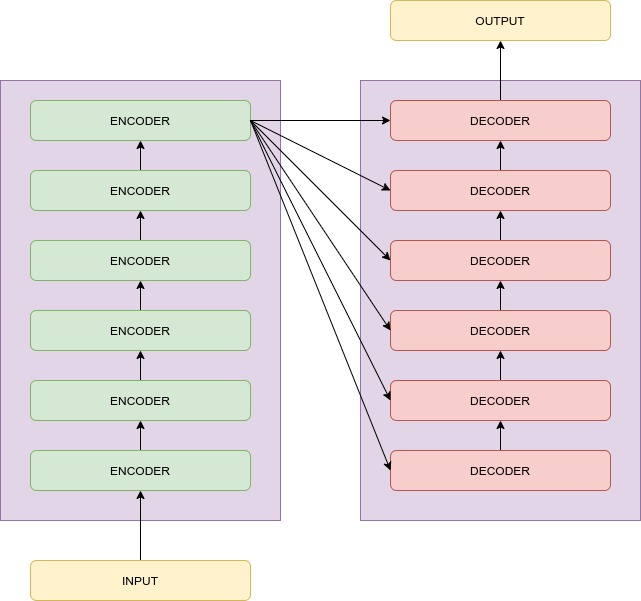
\includegraphics[scale=0.35]{images/bart}
	\caption{\emph{BART} architecture.}
	\label{fig:bart}
\end{figure}
\paragraph{}
The training used for \emph{BART} is based on the mask training used by \emph{BERT} but with a few variations. The model is optimized based on a loss function obtained between the output of the \emph{decoder} and the original text, that is ``corrupted'' with different transformations to make a noised input, forcing the model to capture the language information in an extremely way to understand the noisy input.
\paragraph{}
Among the different ways of ``corrupting'' the text, some of the are:
\begin{itemize}
\item \emph{Token} masking. \\ Same as \emph{BERT}, it masks random \emph{tokens}.
\item \emph{Tokens} removal. \\ In addition to the mask of different \emph{tokens}, \emph{BART} also remove them, thus it has to learn not only to replace the masked \emph{tokens} with the original ones, but also to recognize is some \emph{tokens} are missing and, in that case, to predict which one was the original \emph{token}.
\item \emph{Spans} masking. \\ \emph{BART} not only mask single \emph{tokens}, but also text \emph{spans} are completely masked with a single \emph{[MASK] token}. This way, \emph{BART} has to learn if the mask \emph{token} was a single word or a text \emph{span}. 
\item Sentence permutation. \\ Sentences are randomly shuffled to make the model to learn the real order of the sentences.
\item Document rotation. \\ A random \emph{token} is chosen to rotate the document in a way that it begins with that token, making \emph{BART} to learn to recognize the real start of the document.
\end{itemize}
This way, \emph{BART} trains with highly noised documents and it has to learn to reconstruct them, allowing it to reach a high understanding of the language and to execute different \emph{NLP} tasks, like \emph{QA} or \emph{TS}.
\subsubsection{ProphetNet}
\noindent Another interesting approach is the one proposed by Yan et al.\cite{Yan2020} \emph{ProphetNet} is a novel architecture based also on \emph{encoder-decoder} but, instead of predicting just the next \emph{token} its trained to predict the $n$ next \emph{tokens}.
\paragraph{}
This way, authors say that the overfitting in near words is avoiding as also its the underfitting in far away ones, because in traditional \emph{LM} to predict the next \emph{token} the model focus only on near words, loosing therefore the information provided by \emph{tokens} far away.
\paragraph{}
But in some \emph{NLP} tasks  such \emph{TS} and when dealing with large texts all the context is important for the result, making \emph{ProphetNet} an interesting approach.
\subsubsection{ELECTRA}
Clark et al. propose \emph{ELECTRA} (Efficiency Learning an Encoder that Classifies Tokens Replacements Accurately).\cite{Clark2020} Instead of using the mask training like \emph{BERT} (and so others \emph{LM}), \emph{ELECTRA} uses a novel training way.
\paragraph{}
Instead of replace random \emph{tokens} with a \emph{[MASK] token} (as \emph{MLM} use to do), \emph{ELECTRA} replace them with plausible alternatives by using a ``generator'' (another \emph{MLM}). This way the ``discriminator'' tries to recognize the replaced \emph{tokens}, classifying them as ``original'' or ``replaced'', Figure \ref{fig:electra}. This training reminds to the Generative Adversarial Networks used in Computer Vision tasks, in which two neural networks compete, one of them generates fake images and the other one has to recognize the fake images from a set with real samples.
\begin{figure}[h!]
	\centering
	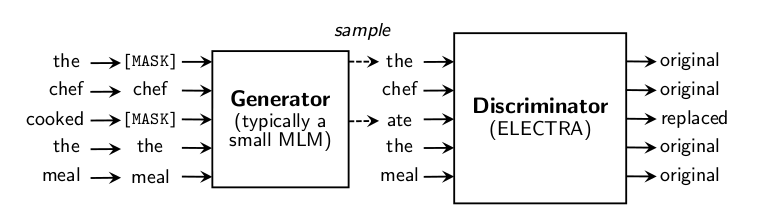
\includegraphics[scale=0.45]{images/electra}
	\caption{\emph{ELECTRA} architecture.}
	\label{fig:electra}
\end{figure}
\paragraph{}
Therefore, \emph{ELECTRA} trains with every single \emph{token} within the document, not only with those that has been masked like the rest of \emph{MLM} do. This makes that \emph{ELECTRA} is able to understand the language before than other \emph{LM} in a more efficient way Figure \ref{fig:compare-electra}.
\begin{figure}[h!]
	\centering
	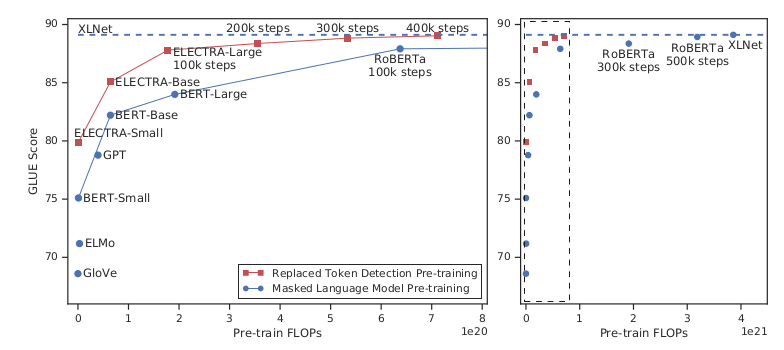
\includegraphics[scale=0.45]{images/compareelectra}
	\caption{Comparison of \emph{ELECTRA} with other \emph{LM}.}
	\label{fig:compare-electra}
\end{figure}
\paragraph{}
This training has allowed that \emph{ELECTRA} reaches state-of-the-art results and, as can be seen in Figure \ref{fig:compare-electra}, in an efficient way. 
\todo{ALBERT}
\todo{LUKE}
\section{Question Answering}
\label{sec:QuestionAnswering}
\noindent Since the beginning of the \emph{NLP}, one of the task most studied and researched is the ability to retrieve information based on a simple query, which is know as Information Retrieval (\emph{IR}). This helps people to find any kind of information in the vast amount of data that is being recollected day to day. For example, search engines like \emph{Google}, are not more than a system of \emph{IR} able to find the documents (web pages) that are more related to the query.
\paragraph{}
But most of the time what people wants is not the whole document but a concise answer to a specific question. This is what the Question Answering tries to solve. Given a question over a context, the \emph{QA} systems try to gives an answer to the user. This context use to be a document that could have been retrieved by an \emph{IR} system, but it's only a document, not a collection of them.
\paragraph{}
This has made possible to search engines and intelligent assistants to improve its performance and to understand the user, improving therefore the user experience with this kind of systems. In Figure \ref{fig:google} it can be seen how the search engine \emph{Google} answers a given question with a concise answer.
\begin{figure}[!h]
	\centering
	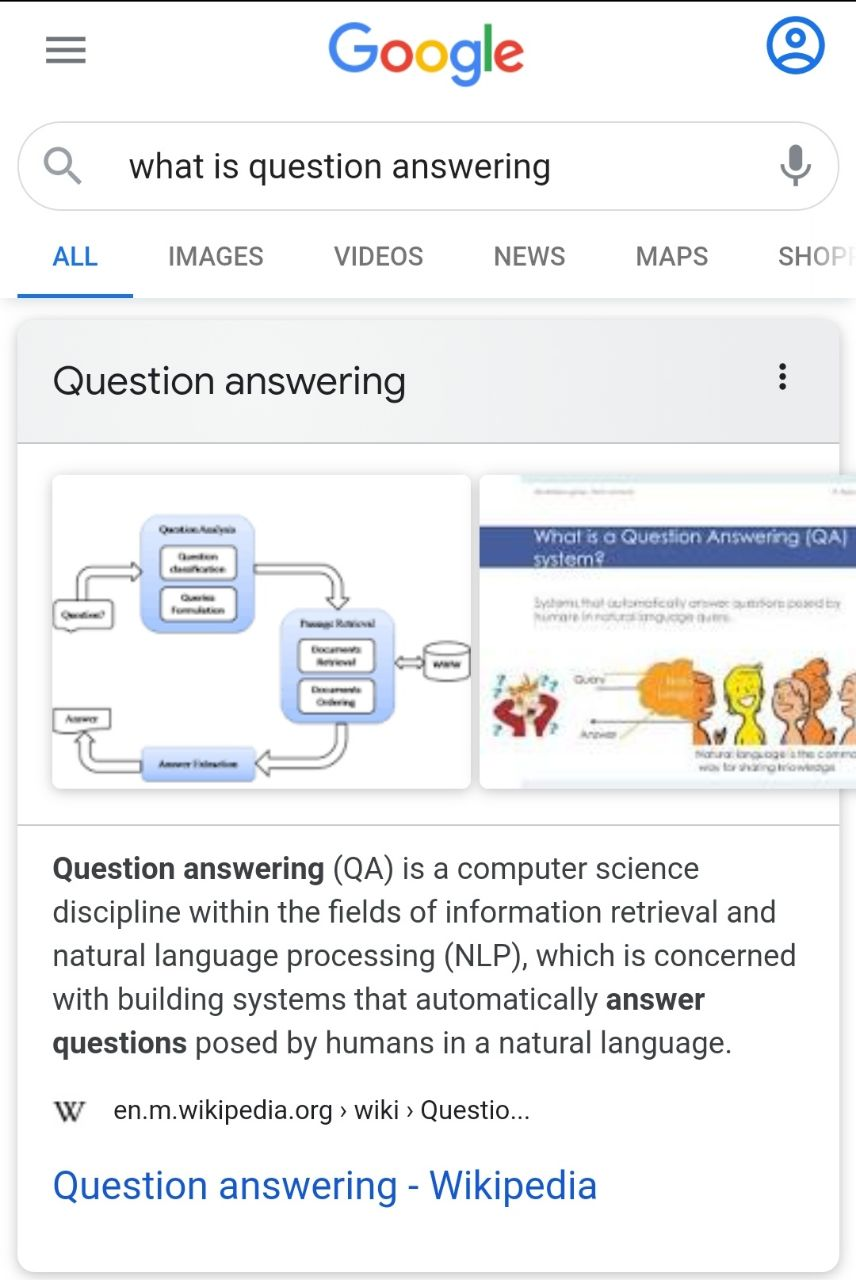
\includegraphics[scale=0.15]{images/google}
	\caption{Question Answering system working in the search engine \emph{Google}.}
	\label{fig:google}
\end{figure}
\paragraph{}
These systems are able to give the answer not only in a written form, but also verbally, and giving also the reference of the document where the answer has been found, in this case \emph{Wikipedia}. As these systems result to be really useful and interesting, both the research and the company fields focused on this task. For instance, the \emph{QA} task was included in the \emph{TREC}, Text REtrieval Conference, or the released of the \emph{Watson} system by \emph{IBM}.
\paragraph{}
Along the history of the \emph{QA} systems there have been proposed different architectures for tese systems, but all of them share some modules that are common in all the systems, as Gonzalez pointed \cite{Gonzalez2003}. These basic modules can be seen in Figure \ref{fig:qa-modules}.
\begin{figure}[!h]
	\centering
	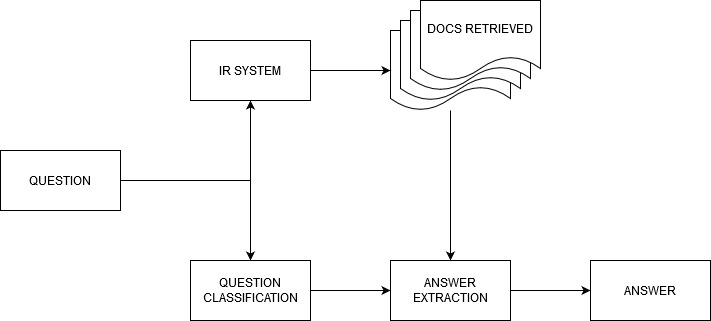
\includegraphics[scale=0.35]{images/qamodules}
	\caption{Question Answering common modules.}
	\label{fig:qa-modules}
\end{figure}
\paragraph{}
The basic workflow in \emph{QA} systems is as follows: 
\begin{enumerate}
\item An \emph{IR} system retrieves the most relevant documents, meanwhile the question is analyzed and classified. The question is classified into different types (e.g.: yes/no question, year-expected, etc) to know what kind of answer is expected (a name, a year, an affirmation or negation, etc).
\item Once it is known the type of answer expected by the question and the most relevant documents have been retrieved, the question is searched within each of the documents. If the answer is found it can be returned to the user or it can be weighted in case there are more than one answer found.
\end{enumerate} 
\paragraph{}
These modules are expanded (or reduced) in some approaches, like for instance in \cite{Ahmed2016a}, where a sub-module is added to the \emph{IR} module. This new sub-module, the \emph{passage retrieval}, is in charge of retrieve the passage within the document that is related to the question. This way, the \emph{answer extractor} module has to look for the answer not in the whole document, but in the related passages. This can be good, less text means less computational and temporal cost, or bad(less text could mean worse performance, because if the \emph{passage retrieval} fails and do not retrieve the passage the answer is located in, the \emph{answer extraction} is not going to be able to find it. But, if the module works as expected, less text will mean also less noise to the \emph{answer extraction} module, which could improve the performance of the system.
\begin{figure}[!h]
	\centering
	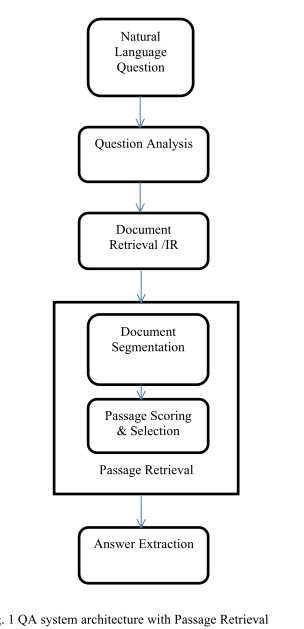
\includegraphics[scale=0.35]{images/ahmed2016}
	\caption{Workflow proposed by Ahmed.}
	\label{fig:ahmed}
\end{figure}
\paragraph{}
This \emph{passage retrieval} module was used in multiple approaches, like the one proposed in \cite{Pablo-Sanchez}, and it was a single task in \emph{TREC} before the \emph{QA} task. 
\paragraph{}
But, with the appearance of the \emph{Transformer} architecture, these modules has changed and modules like \emph{question classification} has even been removed. This module classified the question to know what kind of answer was expected. Along the different \emph{TREC} conferences there have been proposed a los of taxonomies of question and answers types, like the proposed by Moldovan et al. in \cite{Moldovan2001} for the \emph{TREC-8}, the one proposed by Li and Roth for the \emph{TREC-10}\cite{Li2002} or the proposed by Radev et al. in \cite{Radev2005}, Table \ref{tab:radev}.
\begin{table}
	\centering
	\begin{tabular}{|c|c|c|}
		\hline 
		PERSON & PLACE & DATE \\ 
		\hline 
		NUMBER & DEFINITION & ORGANIZATION \\ 
		\hline 
		DESCRIPTION & ABBREVIATION & KNOWNFOR \\ 
		\hline 
		RATE & LENGTH & MONEY \\ 
		\hline 
		REASON & DURATION & PURPOSE \\ 
		\hline 
		NOMINAL & OTHER &  \\ 
		\hline 
	\end{tabular} 
	\caption{Taxonomy proposed by Radev et al.}
	\label{tab:radev}
\end{table}
\paragraph{}
There are also different types of \emph{Question Answering} systems based on the structure of the problem. Some of the time the system is given just a document and a question, and it has to look for the answer to the question within the document, extracting the \emph{span} of text that answers the question and this is why these systems are known as \emph{Extractive Question Answering}. 
\paragraph{}
However, sometimes there are a few options and the model has to choose which one is the correct answer to the question, what is known as \emph{Multiple-Choice}.
\paragraph{}
But both of them have the same objective, to find an answer to a question. The first type, the \emph{Extractive QA} has to find for the \emph{span} of text that answers the question. This way, it is able to find the question within the text but, on the other hand, it can only answer with the \emph{span} extracted and it is not able to answer applying \emph{common-sense} and, for instance, they're not able to answer with a ``yes'' or ``no'', they can only extract the span more related to the expected answer by the question.
\paragraph{}
In the second type, the \emph{Multiple-Choice} problems are able to apply some \emph{common-sense}, being able to answer ``yes/no'' questions, relating countries with cities, languages and so on, but they can only choose between the options given, without being able to find the answer by themselves.
\subsection{Evaluation of QA systems}
\label{sec:qa-evaluation}
The same way that there are different types of \emph{QA} systems, there are also different evaluation metrics. The beginning of the \emph{QA} systems can be traced to 1999, when the \emph{TREC-8} has a specific track for \emph{QA}. In this track, competitors had to propose different approaches to give a concise answer to a given question that was chosen from different sources, from question asked by the competitors their-selves to question obtained from the \emph{FAQFinder} system.
\paragraph{}
At the end, the systems were evaluated, in this case a manual evaluation was carried out, this is, were humans the ones that evaluated. As is explained in \cite{Voorhees1999}, several problems were found while evaluating the systems, with even humans doubting about which one was the correct answer.
\paragraph{}
For instance, one of the doubts was if it would be considered as right in questions about a person just the full name, or if the name or the last-name should be considered as right, or if a list of different names is returned, in which the correct name is contained, but the user don't know for sure which one is.
\paragraph{}
Because of this, they came to the conclusion that, to an answer being considered as right, this should answer the question without any doubt, this is, without having to read the document to know the full answer.
\paragraph{}
Some of the criteria used to consider the answer as right are the next ones:\cite{Allam2012}
\begin{itemize}
\item Relevance: The answer returned should be a response to the question.
\item Correctness: The answer should be factually correct.
\item Conciseness: The answer should not contain extraneous or irrelevant information.
\item Completeness: The answer should be complete (not a part of the answer).
\item Justification: The answer should be supplied with sufficient context to allow a user to determine why this was chosen as an answer to the question.
\end{itemize}
Based on these concepts the answers are classified into different types, as explained in \cite{Allam2012} and \cite{Pablo-Sanchez}:
\begin{itemize}
\item Correct answer.
\item Failed answer.
\item Inexact answer (irrelevant content or missing data).
\item Unsupported answer (not supported by other documents).
\end{itemize}
With these criteria the doubts commented before are solved, for instance, the fact that the answer is not complete (the problem of the names), the fact that the answer alone must be enough for the user without other sources or that the answer should be concise (for example, not returning a list of multiple names).
\paragraph{}
These evaluation metrics have also evolved and nowadays, even though the manual evaluation carried out by humans is still used in some articles, the most common is to evaluate the systems in an automatic way, like the \emph{precision}, the \emph{recall} or the \emph{f1-score}. But other metrics less known have been used, like the ones used in the conferences \emph{TREC-8} and \emph{TREC-11}, the \emph{Mean Reciprocal Rank (MRR)} and the \emph{Confidence Weighted Score (CWS)} respectively, that are defined as:
\begin{equation}
MRR = \sum_{i=1}^{n}\frac{1}{r_{i}}
\label{eq:mrr}
\end{equation}
Where $n$ is the number of questions and $r_{i}$ is the \emph{rank-value} of the first correct answer for the $i$th question.
\begin{equation}
CWS = \sum_{i=1}^{n}\frac{p_{i}}{n}
\label{eq:cws}
\end{equation}
With $n$ being the number of questions and $p_{i}$ the \emph{precision} of the answers from the 1 to the $i$ in a sorted list of answers.
\paragraph{}
Meanwhile the \emph{Multiple-Choice} problems are easily assessable, because can be treated as classification problems, but the \emph{Extractive QA} systems are more complicated to evaluate, because there can be more than one \emph{span} within the text could be a correct answer from the question. Systems also can return the correct labeled \emph{span} but with some added words or without all of them, but being still a correct answer.
\paragraph{}
Anyway, to be able to evaluate these systems in an automatic way, several \emph{datasets} were made.
\subsection{Datasets of QA}
\label{sec:qa-datasets}
To be able to train these systems, there is need a group of questions with their correct answer and the contest, as well as to evaluate them. Therefore, a lot of \emph{datasets} have been developed. Some of the most famous are the next ones:
\subsubsection{SQuAD}
\label{sec:squad}
The \emph{SQuAD} (Sanford QUestion Answering Dataset)\cite{Rajpurkar2016} is a \emph{dataset} created by Rajpurkar et al. in 2016 for \emph{Extractive QA}. It consists of more than 107.785 questions asked over 536 different \emph{Wikipedia} articles by crowdworkers. Given a \emph{Wikipedia} article they have to post a question about the text that the answer is a \emph{span} of text included in the article.
\paragraph{}
To collect the \emph{dataset} the authors used Project Nayuki's \emph{Wikipedia's} internal \emph{PageRanks} to obtain the top 10000 articles of English \emph{Wikipedia}. Then, they select 536 random articles from them and removed figures, tables, short paragraphs, etc. The finally get a set of 23.215 paragraphs for that 536 articles of different topics. Finally they splitted the \emph{dataset} into a training set (80\%), a development set (10\%) and a test set (10\%).
\paragraph{}
Once the articles had been recollected, they employed crowdworkers (like \emph{Amazon Mechanical Turk}) to create the questions and its answers. 
\paragraph{}
Authors then analyzed the question types, the difficulty of the question and the degree of syntactic divergence between the question and the answer. Table \ref{tab:squad-types} shows the different question types and its percentage of appearance in the \emph{dataset}. A complete and official analysis of the \emph{dataset} can be found in \cite{Rajpurkar2016}.
\begin{table}[!h]
	\centering
	\begin{tabular}{|c|c|}
	\hline 
	Answer Type & Percentage (\%) \\ 
	\hline 
	Date  & 8.9\% \\ 
	\hline 
	Other Numeric & 10.9\% \\ 
	\hline 
	Person & 12.9\% \\ 
	\hline 
	Location & 4.4\% \\ 
	\hline 
	Other Entity & 15.3\% \\ 
	\hline 
	Common Noun Phrase & 31.8\% \\ 
	\hline 
	Adjective Phrase & 3.9\% \\ 
	\hline 
	Verb Phrase & 5.5\% \\ 
	\hline 
	Clause & 3.7\% \\ 
	\hline 
	Other & 2.7\% \\ 
	\hline 
	\end{tabular} 
	\caption{Diversity of questions in \emph{SQuAD}.}
	\label{tab:squad-types}
\end{table}
\paragraph{}
To evaluate the systems two different metrics are used over a clean answer (removing punctuation, articles, etc):
\begin{itemize}
	\item Exact match (\emph{EM}): \\
		If the answer matches exactly with any of the ground-truth answers.
	\item \emph{f1-score} (\emph{F1}): \\
		Considering the answer and the ground-truth answers as a bag of words, the \emph{f1-score} is computed between them to measure the average overlap.
\end{itemize}
Authors baseline\cite{Rajpurkar2016} (consisted on window sliding) got a 13.0\% in \emph{EM} and 20\% in \emph{F1} (both of them in test set). A \emph{Logistic Regression} got 40.4\% and 51\% respectively and human performance gets 77\% and 86.8\%.
\paragraph{}
Rightnow, the top \#1 benchmark for \emph{SQuAD} is \emph{LUKE}\cite{Yamada2020} by Yamada et al. that gets a 90.2\% in \emph{EM} and 95.4\% in \emph{F1}.
\paragraph{}
But models trained only on this \emph{dataset} have a problem. If the question is not answerable within the context they make an unreliable response anyway. To solve this \emph{SQuAD} was updated to \emph{SQuADv2}\cite{Rajpurkar2018} with more than 50.000 questions that are indeed not answerable. This way, models have to know when they can answer a question and when they can not.
\paragraph{}
With the same metrics the new human performance is 86.8\% in \emph{EM} and 89.4\% in \emph{F1}. Top \#1 model is \emph{SA-Net on Albert (ensemble)} and gets 90.724\% in \emph{EM} and 93.011\% in \emph{F1}.
\subsubsection{RACE}
\label{sec:race}
\emph{RACE} (Large-scale ReAding Comprehension Dataset From Examinations)\cite{Lai2017} is a \emph{dataset} created by Lai et al. in 2017 for \emph{Multiple-Choice QA}. It consists of near 28.000 passages and near 100.000 questions with 4 possible options each. These questions and passages were collected from English exams for middle and high school Chinese students in the age range between 12 to 18. This way, questions were made by English teachers to enhance and measure the English knowledge of the students, so they cover different topics and are designed to require a high level of reading comprehension and reasoning. 
\paragraph{}
As \emph{RACE} covers a wide range of ages (12-18), the authors splitted it into \emph{RACE-M} and \emph{RACE-H}. \emph{RACE-M} denotes the passages and questions collected from the middle schools students (12-15 years old), meanwhile \emph{RACE-H} denotes the ones collected from the high schools students (15-18 years old). Then bot of them were splitted into training set (90\%), development set (5\%) and test set (5\%). Table \ref{tab:race-sets} shows the number of passages and questions in each with a total number of passages of 27.933 and 97.687 different questions.
\begin{table}[!h]
	\begin{tabular}{|c|ccc|ccc|ccc|}
	\hline 
	Dataset &  & \emph{RACE-M} &  &  & \emph{RACE-H} &  &  & \emph{RACE} & \\ 
	\hline 
	Subset & Train & Dev & Test & Train & Dev & Test & Train & Dev & Test \\ 
	\hline 
	\# passages & 6.409 & 368 & 362 & 18.728 & 1.021 & 1.045 & 25.137 & 1.389 & 1.407 \\ 
	\hline 
	\# questions & 25.421 & 1.436 & 1.436 & 62.445 & 3.451 & 3.498 & 87.866 & 4.887 & 4.934 \\ 
	\hline 
	\end{tabular} 
	\caption{Number of passages and questions in each \emph{RACE} set.}
	\label{tab:race-sets}
\end{table}
\paragraph{}
As it can be seen the number of passages and questions is much larger in the \emph{RACE-H} set, the same as the vocabulary size and the length of the passages, questions and options. Although the vocabulary size is large (136.629), authors note that as the passages and questions have been collected from English exams to Chinese students the vocabulary is not as complex as in other \emph{datasets} where data is collected from news, \emph{Wikipedia} or other sources. 
\paragraph{}
To understand the reading comprehension and reasoning required by \emph{RACE} authors analyzed the \emph{dataset} ``classifying'' the questions into:
\begin{itemize}
	\item Word  matching: The  question  exactly matches a span in the article. The answer is self-evident.
	\item Paraphrasing: The question is entailed or paraphrased by exactly one sentence in the passage. The answer can be extracted within the sentence.
	\item Single-sentence reasoning: The answer could be inferred from a single sentence of the article by recognizing incomplete information or conceptual overlap.
	\item Multi-sentence reasoning: The answer must be inferred from synthesizing information distributed across multiple sentences.
	\item Insufficient/Ambiguous: The question has no answer or the answer is not unique based on the given passage.
\end{itemize}
And, more specifically into:
\begin{itemize}
\item Detail reasoning: to answer the question, the agent should be clear about the details of the pas-sage. The answer appears in the passage but it can-not be found by simply matching the question with the passage. 
\item Whole-picture reasoning: the agent needs to understand the whole picture of the story to obtain the correct answer. 
\item Passage summarization: The question requires the agent to select the best summarization of the passage among four candidate summarizations. 
\item Attitude analysis: The question asks about the opinions/attitudes of the author or a character in the story towards somebody or something
\item World knowledge: Certain external knowledge is needed like simple arithmetic, geography, etc.
\end{itemize}
\paragraph{}
A complete analysis and different methods can be found in \cite{Lai2017}. In the article authors compare human performance with the results of different methods such as windows sliding or \emph{Stanford AR}. The human performance is 95.4\% for \emph{RACE-M} and 94.2\% for \emph{RACE-H}. The top \#1 right now is \emph{Megatron-BERT (ensemble)}\cite{Shoeybi2019} by Shoeybi et al. from \emph{Nvidia}, that achieves an accuracy of 93.1\% for \emph{RACE-H}	and 90.0\% for \emph{RACE-M}.
\subsubsection{QuAIL}
\label{sec:quail}
\emph{QuAIL} (Getting Closer to AI-complete Question Answering: A Set of Prerequisite Real Tasks)\cite{Rogers2020} is a \emph{dataset} created by Rogers et al. in 2020 for \emph{Multiple-Choice QA}. In the article, authors say that although there are several \emph{datasets} for different reasoning tasks (such \emph{QA}), most of them get ``solved'' almost immediately, and this is because of the poor diversity of the data, that has bias and spurious patterns that make the models to recognize these patterns more than to actually learn the language. To solve this, the authors have analyzed different \emph{datasets} and have balanced different types of data to try to reduce the amount of bias and spouring patterns.
\paragraph{}
This has led the authors to find that, for instance, paraphrasing makes models to miss performance, even for \emph{BERT} and other \emph{LM}.
\paragraph{}
\emph{QuAIL} is a multi-domain \emph{dataset} with 200 texts for each of the 4 domains available. Questions about these texts have 3 different options and one \emph{Not Enough Information (NEI)} question, that it's the correct option for unanswerable questions. The texts are from 4 different domains: CC license fiction, Voice of America news, blogs and user stories from Quora and each one has 18 question (\~14k questions). The question are classified into the next types:
\begin{itemize}
	\item Text-based questions: Those questions that the information needed to answer should be found in the text.
	\begin{itemize}
		\item Reasoning about factual information in the text.
		\item Temporal order of events.
		\item Character identity.
	\end{itemize}
	\item Word knowledge questions: Those questions that the answer rely on some kind of inference about characters and events, based on information in the text and world knowledge.
	\begin{itemize}
		\item Causality.
		\item Properties and qualities of characters.
		\item Belief states.
		\item Subsequent state after the narrated events.
		\item Duration of events.
	\end{itemize}
	\item Unanswerable questions. 
\end{itemize}
To avoid some possible co-occurrence of words the authors performed paraphrasing in a total number of 556 questions of 30 fiction texts, aiming in particular to reduce lexical co-occurrences between the text and the words in the question and the correct answer. Results showed that all models suffered a significant drop in performance, specially for \emph{BERT}.
\paragraph{}
The official benchmark\footnote{\url{http://text-machine.cs.uml.edu/lab2/projects/quail/}} shows that only the authors have submitted their models, so it's not possible to compare models yet, but the top \#1 of the leader-board is for the model \emph{TML BERT Baseline} with a 53.4\% for all questions.
\todo{SWAG}
\todo{ARC}
\section{Explainability}
\label{sec:Explainability}
\noindent Deep Learning systems are highly used among society and most of the companies nowadays. These technologies have revolutionized the global thinking of business, allowing to make efficient processes and to solve new tasks unthinkable until now like those involving language understanding. Undoubtedly \emph{AI} systems offer huge benefits and enhance a large number of human activities, however, the use of these systems in some critical business processes like people hiring or credit granting are huge decisions and it is not clear how the model is making these decisions and what are the features in which the model is trusting in order to make the predictions. This way, the effectiveness and insights obtained by the models are limited due to the inability to explain the decisions taken by the models and the repercussion that those decisions may have on the users.
\paragraph{}
This fact has created many concerns about the risks that they introduce and has reduced the initial excitement about the transformation and improvements introduced by these systems. Concerns that have been raised include possible lack of algorithmic fairness (leading to discriminatory decisions), potential manipulation of users, potential lack of inclusiveness, infringement of consumer privacy, and related safety and cybersecurity risks. The use of artificial intelligence explainability (\emph{XAI}) can solve these concerns and provide several business benefits such as:
\begin{itemize}
\item Explanations can help to identify problems in data and features so it can improve the model performance at the same time that can help to better decision making thanks to the additional information provided.
\item Gives a sense of control and safety since the \emph{AI} system owner knows in every moment how the behavior is and each decision can be subjected to pass through safety guidelines and alerts on its violation.
\item One of the main advantages is the possibility to build trust around the model with the stakeholders who can interpret every decision made. Moreover it can monitor ethical issues and violation due to bias in data.
\item Lastly, it can solve compliance issues related with accountability and regulation. (E.g. Adherence to \emph{GDPR} regulation where ``Right to Explain'' is must-have for a system).
\end{itemize}
\emph{XAI} will take more and more importance and a significant part of the effort from the research community and companies will be focused on creating interpretable models or providing a set of tools that help to understand and explain the decisions taken by the \emph{AI} models. The goal is to enable users to understand, trust model predictions while maintaining the learning performance.
\subsection{XAI classification}
\label{sec:xai-classification}
\noindent Although explainability is a recent technique, there are already a lot of different techniques and systems to try to explain models and predictions. Even tough there a lot of techniques, all are based on the same concepts and, therefore, they can be classified depending on their nature in different aspects:
\paragraph{Global Interpretation vs Local Interpretation} Among the different classifications that can be done in order to difference between all the \emph{XAI} techniques, the most important is the type of the explanation. The are two different types of explanations: the explanation of how a model works and the explanation of why a model has given a specific output as a result. 
\paragraph{}
This way, the \emph{Global Interpreters} try to understand the whole model, how it works and what \emph{features} are important for the model to explain the entire model's predictive reasoning. This is very interesting for some use cases, like for instance to understand if the model has some \emph{bias}. On the other hand, the \emph{Local Interpreters} try to explain a unique prediction of the model, by looking at a local subregion in the feature space around the prediction, trying to understand the model decision based on that local region.
\paragraph{Model-specific vs model-agnostic} Other interesting classification of the \emph{XAI} techniques available is to know which ones can be applied to all models or which ones can only be applied to a specific model type. If, for instance, a company has different models being used (e.g. Support Vector Machines, Random Forests and Neural Networks) its more interesting for the company to use the same tool for all models rather than one different technique for each one. Model-specific tools are those one that can be only applied to a specific model type (for instance, those tools that study the \emph{attention} mechanism can only be applied to language models that use \emph{attention}). Model-agnostic, on the other hand, are those tools that can explain every model, no matter its type.
\paragraph{Intrinsic vs post hoc} Simple machine learning models can be explained themselves, this interpretability is considered as intrinsic e.g. rules-based, linear models, parametric models or tree based models. In these types of models the explanation arise itself with the output of the model, and there is no need of post processing to generate an explanation. However, complex models such as Neural Networks require some additional processing to be performed after the predictions are made in order to get the explanation.
\subsection{XAI Techniques}
\noindent Although there are a lot of different techniques available to explain models or predictions, there are some techniques that are the most frequent in the literature. Most of the available tools for \emph{XAI} use these techniques to give the explanation.
	\paragraph{Feature Importance} The model generates the output by performing operations over the inputs, this is, the \emph{features}. Therefore, to understand the importance of the \emph{features} can help to understand the model behavior and to explain it.
	\paragraph{Surrogate Model} If the type of the model is not easily interpretable (such as Neural Networks) or if it is not known, a common way to explain it is to build a second model easily explainable, that will try to behave exactly the way that the model to explain does. This way, by explaining the second model the first one can be explained.
	\paragraph{Example-Driven} This technique is based on search for a similar labeled instance to the input, that will be used as an explanation. These similar instances are obtained from labeled data and they can be gotten by studying semantic similarity, or nearest neighbors in the \emph{feature} space.
	\paragraph{Provenance} In some systems the prediction process involves a series a of reasoning steps, in this cases, the prediction steps can be illustrated to be used as explanation.
	\paragraph{Induction} Some way to explain the model functioning is to generate human-readable representations, such as rules or decision trees that are induced as explanations.
	\paragraph{Anchors} Models use to have some bias in the training data (and therefore in themselves). There are also some inputs that condition an specific output in a way that, if input $x$ is present, the output is always going to be $o$. This is known as an \emph{anchor} and this technique looks for anchors to help to understand a local prediction.
\paragraph{}
These techniques are all based in solving a few operation that enable explainability. Although some of them depend on the type of model being used (\emph{model-specific}, other are applied to any kind of architecture (\emph{model-agnostic}) such as the \emph{Surrogate Model} technique, that usually is trained with \emph{perturbations of the input}\cite{Ribeiro2016} mades by generating random instances modifiying the input $x$. Another technique that can be used with different types of models (althoug it is mostly used with \emph{NN}) is the \emph{first-derivative saliency}, which consists on ``estimate the contribution of input $i$ towards output $o$ by compuing the artial derivative of $o$ with respect to $i$''.\cite{Danilevsky2020}
\paragraph{}
On the other hand, the \emph{model-specific} techniques use to involve some particularities of the model. For instance, if using \emph{RNN}, and more specifically \emph{LSTM}, the output of the \emph{LSTM} cells and the output of the ``gates'' within them can be used to explain the outputs of the model (\emph{Feature Importance} technique, \cite{Ghaeini2018}). More recently, if using \emph{LM} based on \emph{transformers} and/or \emph{attention} layers, the information provided by these layers can be used to explain the behaviour of the model, and because of this there are plenty of works that made use of this startegy, \cite{Luo2018}, \cite{Xie2017}, \cite{Serrano2019}, \cite{Jain2019}.
\subsection{XAI Visualization}
\noindent The main point of \emph{XAI} is to help users and developers to understand the output of a model, why that prediction, why not another one or what can be done to improve the model performance. So, a really important point is to understand the \emph{XAI} techniques outputs, because if the user does not understand the explanation it's not possible that he understands the model behavior. 
\paragraph{}
Because of this, the \emph{XAI} visualization is as important as the techniques used to get the explanation and, therefore, there are a lot of different ways of visualize explanations, depending on the type of the technique used, the model, the kind of the problem (\emph{NLP}, tabular data, computer vision, classification, regression, etc). 
\paragraph{}
\begin{figure}[h]
\centering
\begin{subfigure}{0.3\textwidth}
  \centering
	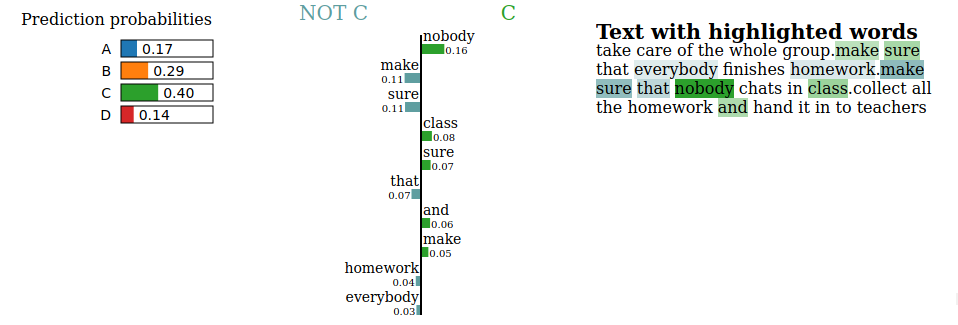
\includegraphics[width=200px]{images/lime-result-2a}
	\caption{Visualization of \emph{LIME}.}
	\label{fig:vis-lime}
\end{subfigure}
\medskip\\
\begin{subfigure}{0.3\textwidth}
  \centering
	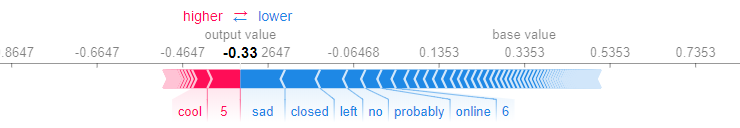
\includegraphics[width=240px]{images/shap}
	\caption{Visualization of \emph{SHAP}.}
	\label{fig:vis-shap}
\end{subfigure}
\medskip\\
\begin{subfigure}{0.45\textwidth}
  \centering
	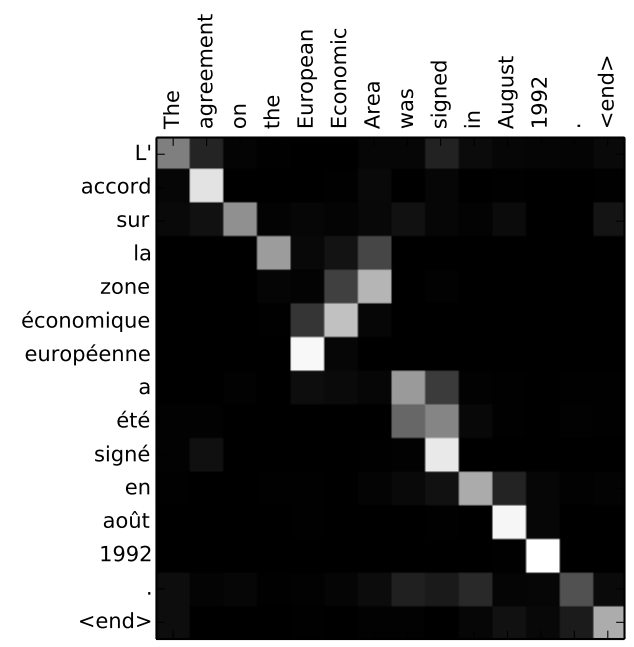
\includegraphics[width=120px]{images/attention}
	\caption{Attention Visualization}
	\label{fig:vis-att}
\end{subfigure}
\begin{subfigure}{0.45\textwidth}
  \centering
	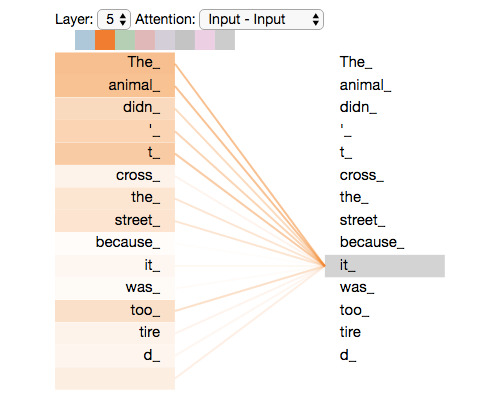
\includegraphics[width=120px]{images/selfattention}
	\caption{\emph{BertVIZ} Visualization.}
	\label{fig:vis-bertviz}
\end{subfigure}
\caption{\emph{XAI} Visualization examples.}
\label{fig:vis-examples}
\end{figure}

\subsection{XAI Evaluation}
\label{xai-evaluation}
\noindent Due to the young age of the \emph{XAI} techniques and to the difficult of the problem being treated, there is no a standard way to evaluate the \emph{XAI} systems and techniques. Most of the papers in the literature that present solutions \cite{Xie2017} don't evaluate the systems and just present a simple discussion and explanation of the \emph{XAI} results based on what the authors think, using only selected examples and not evaluating the system at its whole.
\paragraph{}
Some approaches try to solve this by generating ground truth evaluations to quantify the performance of the \emph{XAI} techniques, by using well known evaluation metrics such as \emph{Precission, Recall and F1-Score}\cite{Carton2018} or \emph{BLEU}\cite{Ling2017}, \cite{Rajani2019}. Although is an interesting way to evaluate the systems, usually there is no only a valid \emph{XAI} explanation, but different explanations may be valid. Because of this, the ground truth acquisition is critic to get a valid evaluation.
\paragraph{}
Other approaches try to solve the problem of multiple valid explanations by using human evaluation. This way, humans can evaluate the quality of the explanations without having to generate ground truth or to measure the similarity of the explanations. This is also interesting, because \emph{XAI} systems try to explain the behavior of a machine learning model, and this is usually a black box humans don't understand and, therefore, can not generate a real ground truth. 
\paragraph{}
Also, as said before, one important step of the \emph{XAI} pipeline is the visualization, and a \emph{XAI} system that can explain the result better to the user is more effective than another one that does not gives a good visualization for explanations understanding, even if this last one has a greater explanation of the model behaviour. This way, the explanations can be evaluated by its understanding of the model prediction and by the human comprehension of the explanations. Lertvittayakumjorn et al. \cite{Lertvittayakumjorn2019} present three different ways of evaluate the \emph{XAI} systems based on the different goals of these systems: To reveal accurately the model behavior; to explain the model predictions; to assist humans in future investigations about uncertain predictions.
\paragraph{}
As \emph{XAI} systems effectiveness depends on the human understanding, is important to have multiple evaluators to deal with different responses and subjectivity, like did Sydorova et al. \cite{Sydorova2019}, where 25 humans evaluated and compared explanations of different techniques.
\paragraph{}
One way mostly used to evaluate the explanations of \emph{attention} layers is to set to zero the maximal entry of the layer to see if the prediction is altered \cite{Serrano2019}. This way, if the result is altered by turning off the dominant weights, this would mean that the weights are indeed explaining the result. Same can be applied to other methods, for instance the replacement of the most important words for a specific prediction could change the result if that are actually important words for the prediction.
\section{Explainabity in NLP}
\label{sec:ExplainabilityNLP}
\noindent The same that has happened with other types of \emph{AI} problems, such as time series regression or in computer vision, has happened to \emph{NLP}, this is, the usage of \emph{Deep Learning} to improve the quality and the results of the models and, with it, the lack of explainability.
\paragraph{}
At the beginning, \emph{NLP} models where mainly based in \emph{white box} techniques, such as \emph{Hidden Markov Models (HMM)}, \emph{Decision Trees} or \emph{Logistic Regressions} which are inherently explainable, but with the arrival and popularity of \emph{Deep Learning} models and \emph{word embeddings} as features, it has become almost impossible to understand why a model gives an output instead of another one. 
\paragraph{}
Because of this, many researchers and companies have focused their research in the explainability, and its application to the \emph{NLP} field, developing systems that are able to explain the model behavior and which features (or word, in case of \emph{NLP}) are more important for the model prediction. But, even tough explainability in \emph{Deep Learning} models is difficult \emph{per se}, and more in \emph{NLP} problems, sometimes it gets even more difficult depending on the problem type.
\paragraph{}
Some \emph{NLP} problems are more complex than others. For instance, text classification problems are less complex than text summarization (depending, of course, on the use case). This is because sometimes there are some words that only appears in some classes, so if that words appear in the text it can be classified without understanding the language. Same happens with simple named entity recognition, where some features like prepositions before the entity, the uppercase and so on help a lot to recognize a named entity. But some problems, like text summarization and question answering are more complex tasks in which the model has to understand the language and the text to be able to solve the task.
\paragraph{}
To understand the language is something really difficult and only humans can do, a lot philosophers say that is language what separates humans from animals actually, and, of course, its complex for machines also. Meanwhile machines are grater than humans while treating with numbers, they can not understand languages as well as humans do, due to the complexity of the task, that involves not only to understand words and grammar, but also to have an understanding about the world, science, politics, history, etc. This makes some tasks really difficult and, although some models have achieved a really good result in some of this tasks, it is not clear if it is because these models understand the language and the task or if it is due to an over-fitting. This can be seen in text summarization, where models trained over scientific papers or over news can not summarize other texts with the same performance, giving as output short sentences (in case of models trained over news), that are not always a good summary.
\paragraph{}
This is why \emph{XAI} is difficult in \emph{NLP} tasks, but also this makes \emph{XAI} important, because if users don't know why the model has given an output, they can not trust in it. However, researcher have been working in explain \emph{NLP} models for the last 5 years, developing really good approaches.
\paragraph{}
In 2015 Voskarides et al.\cite{Voskarides2015} use a two-step approach for automatically explaining relationships between entity pairs, selecting sentences that explain the triplets and using machine learning to rank them according to how they explain the relationship between the entities. Other researchers has also pointed out the utility of applying knowledge graph to deep learning models to increase not only the performance but also the explainability of the models \cite{Palmonari2020}, \cite{Lecue2020}. In 2019, Moon et al. presented \emph{OpenDialKG}\cite{Moon2019}, that use knowledge graph to create a dialogue and reasoning system, that also generates a walk path, providing a way to explain conversational reasoning. 
\paragraph{}
But, although there are a few papers explaining others types of systems such as machine learning algorithms, \cite{Pappas2014}, most of the papers with model-specific techniques are focused on the neural networks due to the difficulty to explain them and their great performance. Gupta et al. proposed a technique named as \emph{Layer-wIse-Semantic-Accumulation (LISA)}, \cite{Gupta2018} for explaining RNN, detecting patterns on while decision making. Poerner et al. developed a method called \emph{LIMSSE}, an adaption of \emph{LIME} to NLP, that achieves good performance in NLP and DNN. Something like that did Wallace et al. \cite{Wallace2018}, using \emph{Deep k-Nearest Neighbors}\cite{Papernot2018} for text classification. As they say in the article, the confidence of neural networks is not a robust measure of model uncertainty, making local interpretation methods less robust in these cases.
\paragraph{}
In 2016, Lei et al. proposed a framework in which they used and encoder and a generator to solve the problem \cite{Lei2016}. The idea is to generate \emph{rationales}, that are pieces of input text as justifications, that once they are feed to the encoder the result of the prediction is the same but that they can help to justify the decision. 
\paragraph{}
Alvarez-Melis et al. proposed a framework to explain black-box models based on input perturbation that returns as explanation a set of input-output tokens that are related to each other inside the model \cite{Alvarez2017}. Input perturbation is one of the techniques most used in \emph{XAI}, but Alvarez-Melis et al. proposed a novel way of generating these perturbations, by using a variational autoencoder to generate similar sentences and, therefore, controlled perturbations. 
\paragraph{}
Another interesting approach is that proposed by Rajani et al. in \cite{Rajani2019}, in which they develop a system named Commonsense Auto-Generated Explanation (\emph{CAGE}) to generate explanations in natural language, by training a model (\emph{GPT-2}) on a new \emph{dataset} called Common Sense Explanations (\emph{CoS-E}).
\todo{Survey of XAI in QA}
\section{Explainability tools}
\label{sec:tools}
\noindent During the past years some tools have been developed to explain (or at least help to understand) machine learning models. Some of these tools can be applied to \emph{LM} and some of them can be applied to \emph{QA} and \emph{Multiple Choice} problems. Next ones are some of the most famous explainability tools.
\subsection{LIME}
\label{sec:Lime}
\noindent \emph{LIME} (Local Interpretations Model-Agnostic Explanations) is a method developed by \emph{Marco Tulio Ribeiro} to explain any black box classifier, with two or more classes.
\paragraph{}
It's able to explain local predictions of almost any machine learning problem, no matter is a computer vision problem, a \emph{NLP} problem or a problem based on tabular data. As it's model-agnostic it's also able to explain every single algorithm, as it considers the model as a black box. 
\paragraph{}
The implementation of this method is available in the \emph{GitHub} of the author \footnote{\url{https://github.com/marcotcr/lime}} with a \emph{BSD-2 Clause license}, so everyone can use the method. This has made this method very famous, being very used by the community. 
The usage of the tool is very easy. Users have to implement a function that takes as input a \emph{NumPy} array with instances and outputs the result of the prediction, with the probability for each class.
 
\paragraph{Advantages:}
\begin{itemize}
	\item Model-agnostic: It can explain any machine/deep learning model.
	\item Easy visualization.
	\item Fast computation.
\end{itemize}
\paragraph{Disadvantages:}
\begin{itemize}
	\item Local: \emph{LIME} is just local explainer, it cannot explain the entire model behavior.
	\item Randomness: score can be different every time as it generates samples randomly so it lacks of consistency.
\end{itemize}

\paragraph{Method Description} This algorithm takes the assumption that is possible to fit a simple interpretable model around a single observation that will mimic how the global model behaves at that locality. This is what makes \emph{LIME} a model-agnostic method, as it will explain the new model created, which is an interpretable model (\emph{RIDGE}), regardless the type of the model to be explained.
\paragraph{}
It works by perturbing the input and seeing how the predictions change for each perturbed input. It first generates a neighborhood data by randomly hiding features (words in this case) from the text instance.  Then, it generates an explanation by approximating the underlying model by an interpretable one learned on the perturbations of the original instance (e.g., removing words).
\paragraph{}
This way, it learns locally weighted linear models on this neighborhood data to explain each of the classes in an interpretable way and indicate the impact of word existence.
\paragraph{}
\begin{figure}
	\centering
	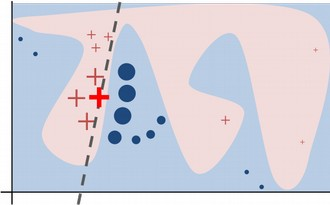
\includegraphics[scale=0.55]{images/lime-explanation}
	\caption{Functioning of \emph{LIME}.}
	\label{fig:lime-ex}
\end{figure}
In the Figure \ref{fig:lime-ex}, the blue/pink background corresponds to the non-linear model being used in the predictions, that has two labels, crosses and circles. While explaining a local predictions (the red cross), \emph{LIME} generates random samples and weights them according to the distance to the prediction being explained (the size of the crosses/circles). The dashes line correspond to the linear model created by \emph{LIME} and its the one being actually explained by \emph{LIME}.

\paragraph{Application to Language Models}
As \emph{LIME} is a model-agnostic method, it's able to explain every type of model, included Language Models. \emph{LIME} is going to consider the original Language Model a black box, creating an additional model, fitted with perturbations of the input. This way, is able to interpret local predictions of Language Models. The perturbations will be made over the instance of the local prediction by, for instance, removing words. 
\paragraph{}
Language Models are based on the prediction of the next word (or sequence), which is more like a regression problem. Even when \emph{LIME} is also able to explain regression problems, is more focused on the classification problems. Nevertheless, the most of the Language Models used nowadays aren't used to predict the next sequence, but to do complex NLP tasks, such as text classification, Named Entity Recognition or Question Answering, and this is done by adding additional layers at the top of the model. This layers will be different depending on the kind of the problem, but most of them can be treated as classification problems. For instance, the Named Entity Recognition problem consists on classify each token as a named entity or not.  This way, \emph{LIME} could be used not only to explain the Language Models themselves, but also the complex model built on top of them, such as \emph{BERT}.

\paragraph{Application to Question Answering}
Question Answering models can be classified into two different types. The ones that try to extract the answer directly from the text, given as the result the tokens inside the text that answer the question (with \emph{datasets} such as \emph{SQuAD}) and the ones that try to select the correct answer among the possible answers given, which are known also as multiple choice problems (with \emph{datasets} such as \emph{RACE}).
\paragraph{} 
Depending on the QA type (extractive or multiple-choice) the way to proceed is different, but both of them can be treated as classification problems. In the extractive ones, span classification layer is added on top on the base model (such as \emph{BERT}), and in the multiple-choice ones  a classification layer is added on top of the pooled output to classify which one is the correct answer.
\paragraph{}
This way, considering the QA problem as a classification one, is easy to adapt \emph{LIME} to use it in this kind of tasks. In these cases, \emph{LIME} can take as input the context, the question, the options or any combination possible between them, explaining for instance which words are important of every single option.

\subsubsection{Attention Heatmap}
\label{sec:AttentionHeatmap}
\noindent One of the most common ways to visualize the \emph{Attention} values is with a heatmap of the values, Fig \ref{fig:vis-att}.
\paragraph{}
The \emph{Attention} method relates each \emph{token} with the others and this methods plots those relationships as a heatmap. This way, it shows the \emph{Attention} value of each \emph{token} in y-axis attending to each \emph{token} in x-axis. But in the \emph{LM} it is common to have multiple heads, so there are two options, to plot a heatmap per each head or to plot a heatmap with an output of all heads at once, that can be the average of the values, the sum, etc.
\paragraph{}
To visualize the \emph{Attention} heatmap is an easy way to see how tokens relate with each others, which may help to understand what is going on inside the model. Although after several experiments (not only of this method but others, as will be seen after) it has been seen that the \emph{Attention} values is not really useful to explain why the model has predict an specific output instead of another one, it can be used, as seen, to detect patterns, useless heads and so on.
\paragraph{}
As an explainability method it is true that it is not as helpful as other methods that are indeed trying to explain the model output. But it can be used to detect if the model is under-fitted (or over-fitted), which may explain a wrong prediction. But it does not help to explain a right prediction.
\paragraph{}
\paragraph{Advantages:}
\begin{itemize}
	\item It allows to visualize the \emph{attention} values easily.
	\item Heatmaps are easily-interpretable visualizations than can make humans to understand model insights in an easy way.
\end{itemize}
\paragraph{Disadvantages:}
\begin{itemize}
	\item It just shows the way \emph{tokens} relate with each other in 2D and between two sentences..
\end{itemize}

\subsubsection{BertViz}
\label{sec:Bertviz}
\noindent \emph{BertViz}, presented by Jesse Vig in 2019 \cite{Vig2019}, is one of the most famous library for visualizing \emph{Attention}  layers. It presents 3 different types of visualization, including:
\begin{itemize}
	\item Head view: Visualize the \emph{attention} patterns in a single layer, Fig \ref{fig:bertviz-head}.
	\item Model view: Visualize the \emph{attention} patterns in every layer at once, Fig \ref{fig:bertviz-model}.
	\item Neuron view: Visualize the \emph{query} and \emph{key} vectors of a single neuron to show how \emph{attention} works, Fig \ref{fig:bertviz-neuron}.
\end{itemize}
\begin{figure}[h]
\centering
\begin{subfigure}{0.4\textwidth}
  \centering
	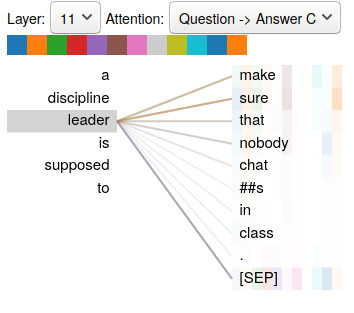
\includegraphics[width=120px]{images/bertviz-question-l11}
	\caption{Head view of \emph{BertViz}.}
	\label{fig:bertviz-head}
\end{subfigure}
\medskip
\begin{subfigure}{0.4\textwidth}
  \centering
	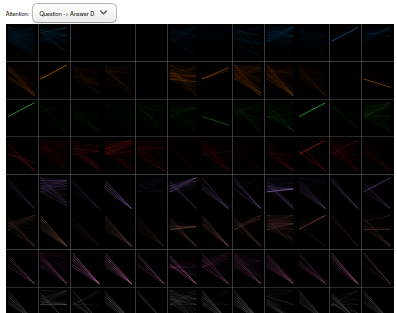
\includegraphics[width=240px]{images/bertviz-model-sample}
	\caption{Model view of \emph{BertViz}.}
	\label{fig:bertviz-model}
\end{subfigure}
\medskip\\
\begin{subfigure}{\textwidth}
	\centering
	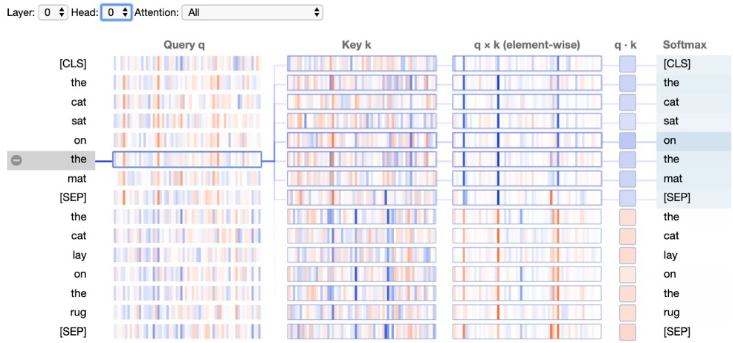
\includegraphics[width=420px]{images/neuronview-example}
	\caption{Neuron view of \emph{BertViz}.}
	\label{fig:bertviz-neuron}
\end{subfigure}
\caption{\emph{BertViz} examples.}
\label{fig:bertviz-examples}
\end{figure}
\paragraph{}
It also supports all models from the \emph{transformers}\footnote{\url{https://github.com/huggingface/transformers}} library of \emph{Huggingface}\footnote{\url{https://huggingface.co/}}, which is the most used library for \emph{transformers} usage and development. This way, it is easy to use the tool and visualize the models used.
\paragraph{}
The implementation of this method is available in the \emph{GitHub} of the author \footnote{\url{https://github.com/jessevig/bertviz}} with a \emph{Apache 2.0 license}, so everyone can use the method even for commercial use. 
\paragraph{}
The usage of the tool is very easy, but depending on the problem. It supports only the visualization between two sentences, and when the input is too large it fails or takes too long to show the result. However, for most of the problems this is enough to see the model behavior.
\paragraph{Advantages:}
\begin{itemize}
	\item It allows to visualize the \emph{attention} in different ways, which makes possible to deep into the model and see how it works.
	\item It supports all models from the \emph{transformers} library, which makes it an easy tool for visualizing the \emph{attention}.
	\item The interactive visualization provided (made with \emph{Javascript}) makes it easy and user-friendly.
\end{itemize}
\paragraph{Disadvantages:}
\begin{itemize}
	\item It only works with two sentences, which is not enough sometimes.
	\item It only works with short inputs.
	\item The Neuron View only supports \emph{BERT}, \emph{GPT-2}, and \emph{RoBERTa} models.
\end{itemize}
\paragraph{Method Description} 
As \emph{BertViz} is only a visualization tool, it does not process anything (like e.g. \emph{LIME}, which has to train a surrogate model).
\paragraph{}
\emph{BertViz} takes the \emph{Attention} weights produced by the model in the \emph{forward} and shows them in pretty and useful way, making simple to understand them. 
\paragraph{}
\begin{figure}
	\centering
	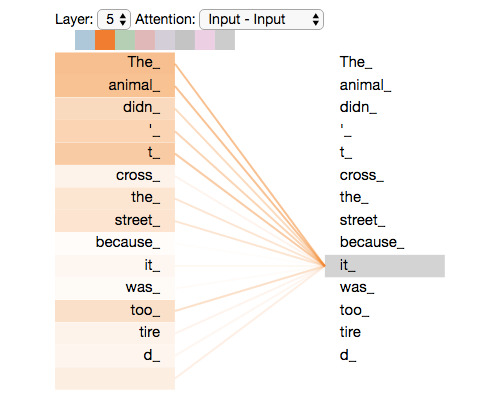
\includegraphics[scale=0.55]{images/selfattention}
	\caption{Example of \emph{BertViz}.}
	\label{fig:bertviz-ex}
\end{figure}
Figure \ref{fig:bertviz-ex} is an example of \emph{BertViz}, in the \emph{Head View}. It shows how \emph{tokens} at left attend to \emph{tokens} at right in one layer (and $n$ heads). The tool provide 5 different options:
\begin{itemize}
	\item All: Shows how all \emph{tokens} attend to every \emph{token}.
	\item Sentence A $\rightarrow$ Sentence A: Shows how \emph{tokens} in Sentence A attend to \emph{tokens} in Sentence A.
	\item Sentence A $\rightarrow$ Sentence B: Shows how \emph{tokens} in Sentence A attend to \emph{tokens} in Sentence B.
	\item Sentence B $\rightarrow$ Sentence B: Shows how \emph{tokens} in Sentence B attend to \emph{tokens} in Sentence B.
	\item Sentence B $\rightarrow$ Sentence A: Shows how \emph{tokens} in Sentence B attend to \emph{tokens} in Sentence A.
\end{itemize}
\paragraph{Application to Question Answering}
By default, \emph{BertViz} does not support \emph{QA} tasks, in the way that it just shows the relation between two sentences. However, it can be considered as Sentence A the question and each option as Sentence B. 
\paragraph{}
This way, some modifications have been developed to make it easier for the user. In these modifications, developed for \emph{Multiple-Choice} problems, the user just has to input the example (including the text, the question and the options) and the modified \emph{BertViz} shows 8 different options:
\begin{itemize}
	\item Question $\rightarrow$ Answer A: Shows how \emph{tokens} in the Question attend to \emph{tokens} in the Answer A.
	\item Question $\rightarrow$ Answer B: Shows how \emph{tokens} in the Question attend to \emph{tokens} in the Answer B.
	\item Question $\rightarrow$ Answer C: Shows how \emph{tokens} in the Question attend to \emph{tokens} in the Answer C.
	\item Question $\rightarrow$ Answer D: Shows how \emph{tokens} in the Question attend to \emph{tokens} in the Answer D.
	\item Answer A $\rightarrow$ Question: Shows how \emph{tokens} in the Answer A attend to \emph{tokens} in the Question.
	\item Answer B $\rightarrow$ Question: Shows how \emph{tokens} in the Answer B attend to \emph{tokens} in the Question.
	\item Answer C $\rightarrow$ Question: Shows how \emph{tokens} in the Answer C attend to \emph{tokens} in the Question.
	\item Answer D $\rightarrow$ Question: Shows how \emph{tokens} in the Answer D attend to \emph{tokens} in the Question.
\end{itemize}
Another modifications were made to show relations regarding \emph{tokens} in the context, but the input in that case was too long for \emph{BertViz}, so it was not possible to show it due to hardware limitations.

\subsection{Intrinsic GPT-3}
\label{sec:gpt3}
\noindent \emph{GPT-3} has demonstrated to be a very powerful model that is able to chat, to answer question, to summarize and even to code functions based on a description of the functionality desired. To do this and to force it to act as expected, it's enough to feed it a few examples with the result expected and then \emph{GPT-3} will generate the output.
\paragraph{}
Therefore, if the user feed it with a few questions (starting by a special \emph{token} \emph{Q:}) with their answers (starting also by a special \emph{token A:}), when the user inputs only a question, the model will generate the answer.
\paragraph{}
Although \emph{GPT-3} has not been trained for any task specifically, it has demonstrated to be able to solve them by an unsupervised zero-shot learning, so it may be able to give an explanation of the answer. 